
\begin{figure}[!htbp]
\begin{center}
\tikzstyle{line} = [thick]
\tikzstyle{arw} = [->, thick,>=stealth,shorten <=2pt, shorten >=2pt]
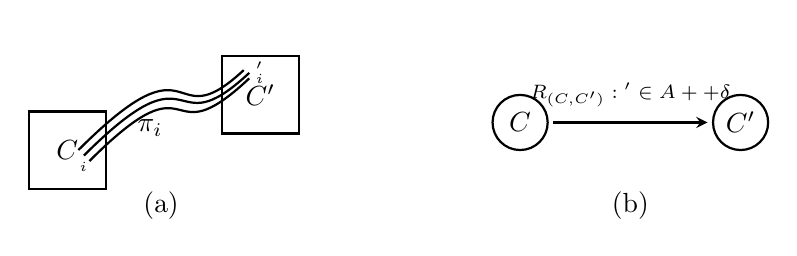
\begin{tikzpicture}
\begin{scope}[scale=0.7]

    \draw [line] (-5.2,-1.2) rectangle (-3.8,0.2);
    \draw [line] (-1.7,-0.2) rectangle (-0.3,1.2);
    \draw [line] (-4.1,-0.7) .. controls +(2.0,2.0) and +(-1.6,-1.5) ..  (-1.2,0.8);
    \draw [line] (-4.2,-0.6) .. controls +(2.1,2.1) and +(-1.5,-1.4) ..  (-1.2,0.9);
    \draw [line] (-4.3,-0.5) .. controls +(2.2,2.2) and +(-1.4,-1.3) ..  (-1.3,0.95);

\node at (-4.5, -0.5) {$C$};
\node at (-1, 0.5) {$C'$};
\node at (-4.2,-0.8) {\scriptsize{$\x_i$}};
\node at (-1.0,0.90) {\scriptsize{$\x_i'$}};
\node at (-3,-0.1) {$\pi_i$};
\node at (-2.8, -1.5) {(a)};
\end{scope}

\begin{scope}[xshift=4.0cm,scale=0.7]
\draw [line] (-2.0,0) circle (0.5);
\draw [line] (2.0,0) circle (0.5);
\draw[arw] (-1.5,0) -- (1.5,0);
\node at (-2.0,0) {$C$};
\node at (2.0,0) {$C'$};
\node at (0,0.5) {\scriptsize{$R_{(C,C')}:\setof{\x' \in A\x + \vb + \delta}$}};
\node at (0.,-1.5) {(b)};
\end{scope}
\end{tikzpicture}
\end{center}
\vspace*{-.3cm}
\caption{(a) Trajectory segments $\traj_i$ are used to compute the
relation $R_{(C,C')}$ that annotates the edge in (b).
$R_{(C,C')}:\setof{\x' \in A\x + \vb + \delta}$ is an interval affine
relation defined by an affine map (matrix $A$ and vector $\vb$) and an
error interval (vector of intervals $\delta$).}
    \label{fig:enriched-edge}
\vspace*{-.3cm}
 \end{figure}
